\documentclass{scrreprt}

\usepackage{aligned-overset}
\usepackage{amsmath}
\usepackage{amsthm}
\usepackage{amssymb}
\usepackage{bm}
\usepackage[inline,shortlabels]{enumitem}
\usepackage{hyperref}
\usepackage[utf8]{inputenc}
\usepackage{multicol}
\usepackage{mathtools}
\usepackage{pdflscape}
\usepackage{physics}
\usepackage{tabularx}
\usepackage[table]{xcolor}
\usepackage{titling}
\usepackage{fancyhdr}
\usepackage{xfrac}
\usepackage{pgfplots}

\pgfplotsset{compat = newest}
\usepgfplotslibrary{fillbetween}
\usetikzlibrary{calc}


\author{Karsten Lehmann}
\date{SoSe 2025}
\title{Übungsblatt 02\\INF-B-260, Informations- und Kodierungstheorie}

\newcommand{\ld}{\text{ld}}

\setlength{\parindent}{0pt}

\setlength{\headheight}{26pt}
\pagestyle{fancy}
\fancyhf{}
\lhead{\thetitle}
\rhead{\theauthor}
\lfoot{\thedate}
\rfoot{Seite \thepage}

\begin{document}
\paragraph{Ü 2 Quellenkodierung}
\begin{enumerate}[1.]
\item Eine diskrete Quelle mit dem Alphabet $X$ und dem Auftritsverhalten
  \[
    \qty(p\qty\big(x_i)) = \qty(
      \frac{1}{8}\;
      \frac{1}{32}\;
      \frac{1}{2}\;
      \frac{1}{16}\;
      \frac{1}{4}\;
      \frac{1}{32}\;
    )
  \]
  sei gegeben.
  Bestimmen Sie die Koderedundanzen bei Binärkodierung nach SHANNON-FANO und
  HUFFMAN.

  \subparagraph{Lsg.} Nach SHANNON-FANO:

  \begin{tabularx}{\textwidth}{|X|X|X|}
    \hline
    $p\qty\big(x_i)$ & Kodierung & Länge $l_i$ \\
    \hline
    $\sfrac{1}{2}$  & 0     & 1 \\
    $\sfrac{1}{4}$  & 10    & 2 \\
    $\sfrac{1}{8}$  & 110   & 3 \\
    $\sfrac{1}{16}$ & 1110  & 4 \\
    $\sfrac{1}{32}$ & 11110 & 5 \\
    $\sfrac{1}{32}$ & 11111 & 5 \\
    \hline
  \end{tabularx}
  Nun ist die mittlere gewichtete Kodewortlänge
  \[
    l_m = \sum_{i = 1}^n p\qty\big(x_i) \cdot l_i \approx 1.94 \frac{\text{KZ}}{\text{QZ}}
  \]
  wobei KZ für Kanalzeichen und QZ für Quellzeichen stehen.

  Weiter ist die (Quellen)Entropie, beziehungsweise der mittlere Informationsgehalt
  \[
    H_m = \sum_{i = 1}^n p\qty\big(x_i) \cdot \ld \frac{1}{p\qty\big(x_i)} = \approx 1.94 \frac{\text{bit}}{\text{QZ}}
  \]

  Schließlich ist die Entropie am Kanaleingang des Übertragungskanals
  \[
    H_K = 1 \frac{\text{bit}}{\text{Kanalzeichen}}
  \]
  Somit ist die Redundanz
  \[
    R_K = l_m \cdot H_K - H_m = 1.94 \frac{\text{KZ}}{\text{QZ}} \cdot 1 \frac{\text{bit}}{\text{Kanalzeichen}} - 1.95 \frac{\text{bit}}{\text{QZ}} = 0 \frac{\text{bit}}{\text{QZ}}
  \]

  \newpage
  Weiter die Kodierung nach HUFFMAN:

  \begin{tikzpicture}
    \node (1) at (0, 0) {$\sfrac{1}{2}$};
    \node (2) at (0, -1) {$\sfrac{1}{4}$};
    \node (3) at (0, -2) {$\sfrac{1}{8}$};
    \node (4) at (0, -3) {$\sfrac{1}{16}$};
    \node (5) at (0, -4) {$\sfrac{1}{32}$};
    \node (6) at (0, -5) {$\sfrac{1}{32}$};

    \node (7) at (2, -4.5) {$\sfrac{1}{16}$};

    \node (8) at (4, -3) {$\sfrac{1}{8}$};

    \node (9) at (6, -2) {$\sfrac{1}{4}$};

    \node (10) at (8, -1) {$\sfrac{1}{2}$};

    \node (11) at (10, 0) {$1$};

    \draw (5) -- node[midway, above] {0} (7);
    \draw (6) -- node[midway, above] {1} (7);

    \draw (4) -- node[midway, above] {0} (8);
    \draw (7) -- node[midway, above] {1} (8);

    \draw (3) -- node[midway, above] {0} (9);
    \draw (8) -- node[midway, above] {1} (9);

    \draw (2) -- node[midway, above] {0} (10);
    \draw (9) -- node[midway, above] {1} (10);

    \draw (1) -- node[midway, above] {0} (11);
    \draw (10) -- node[midway, above] {1} (11);
  \end{tikzpicture}

  Und somit ist der Kode sowie die Länge analog der SHANNON-FANO Kodierung.

\item Eine diskrete Quelle mit dem Alphabet $X$ sei mit dem Auftrittsverhalten
  \[
    \qty(p\qty\big(x_i)) = \qty(
      0.06 \;
      0.12 \;
      0.14 \;
      0.15 \;
      0.30 \;
      0.05 \;
      0.08 \;
      0.10 \;
    )
  \]
  gegeben.
  Bestimmen sie die mittleren Kodewortlängen und Koderedundanzen für die
  \begin{enumerate}[(a)]
  \item Binärkodierung nach SHANNON-FANO

    \subparagraph{Lsg.} Es ist

    \begin{tabularx}{\textwidth}{|X|X|X|}
      \hline
      $p\qty\big(x_i)$ & Kodierung & Länge $l_i$ \\
      \hline
      $0.30$ & 00   & 2 \\
      $0.15$ & 01   & 2 \\
      $0.14$ & 100  & 3 \\
      $0.12$ & 101  & 3 \\
      $0.10$ & 1100 & 4 \\
      $0.08$ & 1101 & 4 \\
      $0.06$ & 1110 & 4 \\
      $0.05$ & 1111 & 4 \\
      \hline
    \end{tabularx}

    Nun ist die mittlere gewichtete Kodewortlänge
    \[
      l_m = \sum_{i = 1}^n p\qty\big(x_i) \cdot l_i = 2.84 \frac{\text{KZ}}{\text{QZ}}
    \]

    Weiter ist die (Quellen)Entropie, beziehungsweise der mittlere Informationsgehalt
    \[
      H_m = \sum_{i = 1}^n p\qty\big(x_i) \cdot \ld \frac{1}{p\qty\big(x_i)} = \approx 2.7 \frac{\text{bit}}{\text{QZ}}
    \]

    Schließlich ist die Entropie am Kanaleingang des Übertragungskanals
    \[
      H_K = 1 \frac{\text{bit}}{\text{Kanalzeichen}}
    \]
    Somit ist die Redundanz
    \[
      R_K = l_m \cdot H_K - H_m = 2.84 \frac{\text{KZ}}{\text{QZ}} \cdot 1 \frac{\text{bit}}{\text{Kanalzeichen}} - 2.78 \frac{\text{bit}}{\text{QZ}} = 0.06 \frac{\text{bit}}{\text{QZ}}
    \]

  \item Binärkodierung nach HUFFMAN

    \subparagraph{Lsg} Es ist

    \begin{tikzpicture}
      \node (1) at (0, 0) {$0.3$};
      \node (2) at (0, -1) {$0.15$};
      \node (3) at (0, -2) {$0.14$};
      \node (4) at (0, -3) {$0.12$};
      \node (5) at (0, -4) {$0.10$};
      \node (6) at (0, -5) {$0.08$};
      \node (7) at (0, -6) {$0.06$};
      \node (8) at (0, -7) {$0.05$};

      \node (9) at (2, -6.5) {$0.11$};
      \node (10) at (2, -4.5) {$0.18$};
      \node (11) at (4, -4.5) {$0.23$};
      \node (12) at (6, -3.5) {$0.41$};
      \node (13) at (6, -1.5) {$0.29$};
      \node (14) at (8, -1) {$0.59$};
      \node (15) at (10, -2) {$1$};

      \draw (7) -- node[midway, above] {0} (9);
      \draw (8) -- node[midway, above] {1} (9);
      \draw (5) -- node[midway, above] {0} (10);
      \draw (6) -- node[midway, above] {1} (10);
      \draw (4) -- node[midway, above] {0} (11);
      \draw (9) -- node[midway, above] {1} (11);
      \draw (10) -- node[midway, above] {0} (12);
      \draw (11) -- node[midway, below] {1} (12);
      \draw (2) -- node[midway, above] {0} (13);
      \draw (3) -- node[midway, below] {1} (13);
      \draw (1) -- node[midway, above] {0} (14);
      \draw (13) -- node[midway, above] {1} (14);
      \draw (14) -- node[midway, above] {0} (15);
      \draw (12) -- node[midway, above] {1} (15);
    \end{tikzpicture}

    Damit ist der Code

    \begin{tabularx}{\textwidth}{|X|X|X|}
      \hline
      $p\qty\big(x_i)$ & Kodierung & Länge $l_i$ \\
      \hline
      $0.30$ & 00   & 2 \\
      $0.15$ & 010  & 3 \\
      $0.14$ & 011  & 3 \\
      $0.12$ & 110  & 3 \\
      $0.10$ & 100  & 3 \\
      $0.08$ & 101  & 3 \\
      $0.06$ & 1110 & 4 \\
      $0.05$ & 1111 & 4 \\
      \hline
    \end{tabularx}

    Und die mittlere gewichtete Kodewortlänge
    \[
      l_m = \sum_{i = 1}^n p\qty\big(x_i) \cdot l_i = 2.81 \frac{\text{KZ}}{\text{QZ}}
    \]

    Weiter ist die (Quellen)Entropie, beziehungsweise der mittlere Informationsgehalt
    analog zu SHANNON-FANO
    \[
      H_m = \sum_{i = 1}^n p\qty\big(x_i) \cdot \ld \frac{1}{p\qty\big(x_i)} = \approx 2.7 \frac{\text{bit}}{\text{QZ}}
    \]

    Schließlich ist die Entropie am Kanaleingang des Übertragungskanals
    \[
      H_K = 1 \frac{\text{bit}}{\text{Kanalzeichen}}
    \]
    Somit ist die Redundanz
    \[
      R_K = l_m \cdot H_K - H_m = 2.81 \frac{\text{KZ}}{\text{QZ}} \cdot 1 \frac{\text{bit}}{\text{Kanalzeichen}} - 2.78 \frac{\text{bit}}{\text{QZ}} = 0.03 \frac{\text{bit}}{\text{QZ}}
    \]

    Dabei ist anzumerken, dass HUFFMAN wohl meistens/immer? besser ist.
  \end{enumerate}

\item Eine diskrete Quelle $X$ mit unterschiedlichen
  Auftrittswahrscheinlichkeiten der Zeichen sei in folgenden Varianten kodiert:

  \begin{enumerate*}[(1)]
  \item
    \begin{tabular}{l}
      $a_1^* = \qty\big(111)$ \\
      $a_2^* = \qty\big(101)$ \\
      $a_3^* = \qty\big(100)$ \\
      $a_4^* = \qty\big(11)$ \\
      $a_5^* = \qty\big(01)$ \\
      $a_6^* = \qty\big(00)$ \\
      $a_7^* = \qty\big(1101)$ \\
      $a_8^* = \qty\big(1110)$ \\
    \end{tabular}

  \item
    \begin{tabular}{l}
      $a_1^* = \qty\big(111)$ \\
      $a_2^* = \qty\big(101)$ \\
      $a_3^* = \qty\big(100)$ \\
      $a_4^* = \qty\big(010)$ \\
      $a_5^* = \qty\big(011)$ \\
      $a_6^* = \qty\big(00)$ \\
      $a_7^* = \qty\big(1101)$ \\
      $a_8^* = \qty\big(1100)$ \\
    \end{tabular}
  \end{enumerate*}

  Prüfen Sie die Dekodierbarkeit beider Kodes und begründen Sie das Ergebnis!

  \subparagraph{Lsg.} Hier genügt es die Präfixfreiheit zu prüfen.
  Dabei fällt direkt auf, dass für die erste Variante zum Beispiel $a_1^4$ ein
  Präfix von $a_1^*$, $a_7^*$ und $a_8^*$ ist.
  Somit kann diese Variante nicht dekodiert werden.

  Die zweite Variante ist hingegen Präfixfrei.

\item Eine diskrete Quelle ist mit $p\qty\big(A) = 0.1$ und $p\qty\big(B) = 0.9$
  gegeben.
  Bestimmen Sie
  \begin{enumerate}[(a)]
  \item die Entropie der Quelle

    \subparagraph{Lsg.} Es ist
    \[
      H_m = \sum_{i = 1}^n p\qty\big(x_i) \cdot \ld \frac{1}{p\qty\big(x_i)} = \approx 0.47 \frac{\text{bit}}{\text{QZ}}
    \]

  \newpage
  \item die Koderedundanz bei Binärkodierung mit
    $l_A = l_B = 1 \frac{\text{KZ}}{\text{QZ}}$

    \subparagraph{Lsg.} Offensichtlich ist $l_m = 1 \frac{\text{KZ}}{\text{QZ}}$ und
    mit
    \[
      H_K = 1 \frac{\text{bit}}{\text{Kanalzeichen}}
    \]
    die Redundanz
    \[
      R_K = l_m \cdot H_K - H_m = 1 \frac{\text{KZ}}{\text{QZ}} \cdot 1 \frac{\text{bit}}{\text{Kanalzeichen}} - 0.47 \frac{\text{bit}}{\text{QZ}} = 0.53 \frac{\text{bit}}{\text{QZ}}
    \]

  \item die Optimalkodierung nach SHANNON-FANO und Koderedundanz bei einer
    erweiterten Quelle mit der Blocklänge $m = 2$.

    \subparagraph{Lsg.} Es sind

    \begin{tabularx}{\textwidth}{|X|X|X|X|X|}
      \hline
      Block & Auftritts-wahrscheinlichkeit $p\qty\big(x_i)$ & Kode & Länge \\
      \hline
      BB & 0.81 & 0   & 1 \\
      AB & 0.09 & 10  & 2 \\
      BA & 0.09 & 110 & 3 \\
      AA & 0.01 & 111 & 3 \\
      \hline
    \end{tabularx}
    Weiter sind
    \[
      l_m^{\qty{2}} = \sum_{i = 1}^n p\qty\big(x_i) \cdot l_i = 1.29 \frac{\text{KZ}}{\text{Block}}
      \text{ und }
      l_m = \frac{1.29 \frac{\text{KZ}}{\text{Block}}}{2 \frac{\text{QZ}}{\text{Block}}} = 0.645 \frac{\text{KZ}}{\text{QZ}}
    \]

    Somit folgt die Redundanz
    \[
      R_K = l_m \cdot H_K - H_m = 0.645 \frac{\text{KZ}}{\text{QZ}} \cdot 1 \frac{\text{bit}}{\text{Kanalzeichen}} - 0.47 \frac{\text{bit}}{\text{QZ}} = 0.175 \frac{\text{bit}}{\text{QZ}}
    \]
  \end{enumerate}
\end{enumerate}

\newpage
\paragraph{Zusatzaufgabe} Sei $X = \qty\big{x_1, x_2, x_3}$ eine Quelle mit den
Auftrittswahrscheinlichkeiten $p\qty\big(x_1) = 0.1$, $p\qty\big(x_2) = 0.5$ und
$p\qty\big(x_3) = 0.4$ für die einzelnen Zeichen.

\begin{enumerate}[(a)]
\item Welche Koderedundanz wird erreicht, wenn die Auftrittswahrscheinlichkeiten
  unberücksichtigt bleiben?

  \subparagraph{Lsg.} Hier wird eine gleichmäßige Kodierung angenommen und somit ist
  \[
    l_m = \left\lceil \ld\qty\big(N) \right\rceil
    = \left\lceil \ld\qty\big(3) \right\rceil
    = \left\lceil 1.67 \right\rceil
    = 2 \frac{\text{KZ}}{\text{QZ}}
  \]
  Weiter ist (wieder mit der richtigen Wahrscheinlichkeit)
  \[
    H_m = \sum_{i = 1}^n p\qty\big(x_i) \cdot \ld \frac{1}{p\qty\big(x_i)} = \approx 1.36 \frac{\text{bit}}{\text{QZ}}
  \]
  und schließlich die Redundanz
  \[
    R_K = l_m \cdot H_K - H_m = 2 \frac{\text{KZ}}{\text{QZ}} \cdot 1 \frac{\text{bit}}{\text{Kanalzeichen}} - 1.36 \frac{\text{bit}}{\text{QZ}} = 0.64 \frac{\text{bit}}{\text{QZ}}
  \]

\item Bestimmen Sie Quellenkodewörter mit einer Kodierung, die eine Koderedundanz
  $R_K \leq 0.1 \frac{\text{bit}}{\text{QZ}}$ besitzt.

  \subparagraph{Lsg.} Mit eine Blocklänge von 2:

  \begin{tabularx}{\textwidth}{|X|X|X|X|X|}
    \hline
    Block & Auftritts-wahrscheinlichkeit $p\qty\big(x_i)$ & Kode & Länge \\
    \hline
    $x_2x_2$ & 0.25 & 00    & 2 \\
    $x_2x_3$ & 0.20 & 010   & 3 \\
    $x_3x_2$ & 0.20 & 100   & 3 \\
    $x_3x_3$ & 0.16 & 110   & 3 \\
    $x_1x_2$ & 0.05 & 111   & 3 \\
    $x_2x_1$ & 0.05 & 101   & 3 \\
    $x_1x_3$ & 0.04 & 1110  & 4 \\
    $x_3x_1$ & 0.04 & 11110 & 5 \\
    $x_1x_1$ & 0.01 & 11111 & 5 \\
    \hline
  \end{tabularx}
  Dabei ist
  \[
    l_m^{\qty{2}} = \sum_{i = 1}^n p\qty\big(x_i) \cdot l_i = 2.89 \frac{\text{KZ}}{\text{Block}}
    \text{ und }
    l_m = \frac{2.89 \frac{\text{KZ}}{\text{Block}}}{2 \frac{\text{QZ}}{\text{Block}}} = 1.445 \frac{\text{KZ}}{\text{QZ}}
  \]
  und die Redundanz
  \[
    R_K = l_m \cdot H_K - H_m = 1.445 \frac{\text{KZ}}{\text{QZ}} \cdot 1 \frac{\text{bit}}{\text{Kanalzeichen}} - 1.36 \frac{\text{bit}}{\text{QZ}} \approx 0.09 \frac{\text{bit}}{\text{QZ}}
  \]
\end{enumerate}

\end{document}
